\begin{exo}
	On considère la figure ci-dessous.
	\begin{center}
		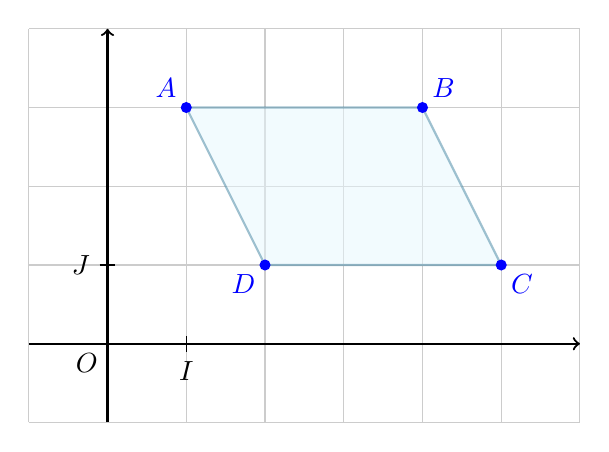
\begin{tikzpicture}
			\draw[gray!40, thin] (-1,-1) grid (6,4);
			\draw[->, thick] (-1,0) -- (6,0);
			\draw[->, thick] (0,-1) -- (0,4);
			\node at (0,0) [below left] {$O$};
			\node at (1,-0.1) [below] {$I$};
			\node at (-0.1,1) [left] {$J$};
			\draw (1,-0.1) -- (1,0.1);
			\draw (-0.1,1) -- (0.1,1);
			\coordinate (A) at (1,3);
			\coordinate (B) at (4,3);
			\coordinate (C) at (5,1);
			\coordinate (D) at (2,1);
			\draw[thick, cyan!60!black, fill=cyan!10, opacity=0.5] (A) -- (B) -- (C) -- (D) -- cycle;
			\foreach \p/\name/\pos in {A/A/above left, B/B/above right, C/C/below right, D/D/below left} {
					\fill[blue] (\p) circle (2pt);
					\node[\pos, blue] at (\p) {$\name$};
				}
		\end{tikzpicture}
	\end{center}

	\begin{enumerate}
		\item Calculer les coordonnées de $K$ milieu de $[AC]$.
		\item Calculer les coordonnées de $L$ milieu de $[BD]$.
		\item En déduire que $ABCD$ est un parallélogramme.
	\end{enumerate}
\end{exo}
